\documentclass[conference]{IEEEtran}
\IEEEoverridecommandlockouts
\usepackage{cite}
\usepackage{mathptmx} % Times for text and mathematics
\usepackage{amsmath,amssymb}
\usepackage{graphicx}
\usepackage{booktabs}
\usepackage{multirow}
\usepackage{array}
\usepackage{algorithm}
\usepackage{algpseudocode}
\usepackage{tikz}
\usetikzlibrary{arrows.meta,positioning,fit,shapes.geometric}
\usepackage[hidelinks]{hyperref}
\usepackage{xcolor}
\def\BibTeX{{\rm B\kern-.05em{\sc i\kern-.025em b}\kern-.08em
    T\kern-.1667em\lower.7ex\hbox{\sc e}\kern-.125emX}}

\begin{document}

\title{\textbf{ScamGuard: AI-Based Online Scam and Fraud\\ Detection System}}

\author{
\IEEEauthorblockN{Dr. Kayarvizhy N}
\IEEEauthorblockA{\textit{Professor} \\ \textit{Department of Computer Science and} \\ \textit{Engineering} \\
\textit{B.M.S. College of Engineering}\\
Bengaluru, India \\
kayarvizhyn.cse@bmsce.ac.in}
\and
\IEEEauthorblockN{Priyam Thakur}
\IEEEauthorblockA{\textit{Department of Computer Science and} \\ \textit{Engineering} \\
\textit{B.M.S. College of Engineering}\\
Bengaluru, India \\
priyamthakur.cs23@bmsce.ac.in}
\and
\IEEEauthorblockN{Bhavya Goyal}
\IEEEauthorblockA{\textit{Department of Computer Science and} \\ \textit{Engineering} \\
\textit{B.M.S. College of Engineering}\\
Bengaluru, India \\
bhavyagoyal.cs23@bmsce.ac.in}
\and
\IEEEauthorblockN{Samir Chaudhary}
\IEEEauthorblockA{\textit{Department of Computer Science and} \\ \textit{Engineering} \\
\textit{B.M.S. College of Engineering}\\
Bengaluru, India \\
samirchaudhary.cs23@bmsce.ac.in}
\and
\IEEEauthorblockN{Sana Subodh}
\IEEEauthorblockA{\textit{Department of Computer Science and} \\ \textit{Engineering} \\
\textit{B.M.S. College of Engineering}\\
Bengaluru, India \\
sanasubodh.cs23@bmsce.ac.in}
}

\maketitle

\begin{abstract}
SMS remains one of the main channels of financial fraud in India. Scam messages copy the look of bank KYC reminders, electricity disconnection notices, parcel updates and traffic challans, and they increasingly arrive in Hindi. Public smishing collections contain only the messages that users chose to report, so they offer no verified genuine class. This paper presents ScamGuard, an AI-based online scam and fraud detection system, together with ScamGuard-IN-2026, the corpus built for it: 11,399 messages drawn from Indian user-reported smishing in the IMC~2025 collection, real Indian genuine SMS, scam texts quoted in 2025--26 advisories, and clearly marked synthetic messages used for training only. All 2,922 reported-message campaigns were checked by rule or by hand, and 19.5\% of the retained reports turned out to be genuine bank alerts, one-time-password messages, order updates or advertisements. Near-duplicate campaigns were grouped with MinHash, and no campaign crosses the train--test boundary. On 1,874 held-out real messages from unseen campaigns, logistic regression over word and character TF-IDF reaches an F1-score of 98.1\% with a 2.6\% false-alarm rate, whereas training on raw report labels raises the false-alarm rate to 34.0\%. The deployed system adds interpretable intent rules that highlight the phrases behind each verdict; it reaches 97.1\% accuracy (95\% CI 96.3--97.8) and scores a message in under 4~ms. We also show that hand-written rules that look strong on the developers' own test messages do not improve accuracy on independent real data. The corpus, audit decisions and code are released.
\end{abstract}

\begin{IEEEkeywords}
smishing, SMS fraud detection, label noise, data leakage, Indian languages, text classification
\end{IEEEkeywords}

\section{Introduction}

SMS remains the most direct way to reach a phone user in India, and fraudsters use it accordingly. In a 2025 measurement study of over 64,000 public smishing reports, most of the sender numbers that could be attributed to an operator belonged to Indian mobile networks~\cite{agarwal2025fishing}. The messages are short, often written in English, Hindi or a mix of the two, and they copy the look of real service messages: a ``KYC update'' from a bank, an electricity disconnection notice, a parcel held for a small fee, a traffic fine with an attached app.

Machine-learning filters for SMS have a long history, but they were built mainly to separate promotional spam from personal chat. The accuracies of 96--99\% reported for that task~\cite{roy2020deep,goel2024ml,ahmadi2025llm} say little about present-day Indian fraud, and a recent systematic review of 119 smishing papers notes that available datasets are ``often limited in scale, diversity, and temporal coverage''~\cite{pritom2026sms}.

Newer corpora help with the scam side. The Smishtank dataset holds 1,062 validated reports~\cite{timko2024smishing}, and the IMC~2025 collection mines tens of thousands of public reports with their scam types~\cite{agarwal2025fishing}. Neither contains a genuine class, and both are built from what users \emph{reported}. The IMC~2025 authors state that reports carry ``no verification or validation''~\cite{agarwal2025fishing}. Our first reading of the Indian subset confirmed the concern: genuine debit alerts, OTP messages that tell the user not to share the code, and ordinary bank advertisements had been reported as smishing alongside real scams.

This matters most for false alarms. A scam filter that flags a user's real bank alert teaches the user to ignore it. Genuine notices are easy to misread: an operator message asking users to report spam to the 1909 helpline uses the same words (\textit{block}, \textit{report}, \textit{number}) as many scams. ScamGuard is designed so that such messages are recognised as genuine and so that every verdict comes with the phrases that caused it.

\textbf{Contributions.} This paper makes four contributions.
\begin{enumerate}
\item \textit{An audited Indian corpus.} We build ScamGuard-IN-2026 from four real sources and a synthetic source used only for training, and we audit every reported-message campaign. We release each labelling decision.
\item \textit{A measurement of report noise.} We quantify how many reported messages are genuine (19.5\% of retained IMC~2025 rows) and what training on report labels does to false alarms (2.6\% rises to 34.0\%).
\item \textit{A leakage-aware protocol.} We group near-duplicate campaigns with MinHash and split by campaign. We report how much a random split overstates performance on the same data.
\item \textit{An honest assessment of hybrid rules.} We compare the classifier alone, hand-weighted intent rules and learned fusion weights on independent real data and on the developers' own challenge messages, and show that the two evaluations disagree.
\end{enumerate}

The remainder of the paper is organised as follows. Section~\ref{sec:related} reviews related work. Section~\ref{sec:problem} states the problem and research questions. Sections~\ref{sec:data} and~\ref{sec:method} describe the corpus and the detector. Section~\ref{sec:setup} gives the experimental setup, Section~\ref{sec:results} the results, and Sections~\ref{sec:discussion}--\ref{sec:conclusion} discuss findings, limitations and ethics.

\section{Related Work}
\label{sec:related}

\subsection{SMS spam filtering}
The SMS Spam Collection~\cite{almeida2011contributions} became the standard benchmark because it was public and labelled. Almeida \textit{et al.} later compared many classifiers on it and preferred a linear SVM, which blocked only 0.18\% of legitimate messages while catching 83.1\% of spam~\cite{almeida2013towards}. Deep models on the same data report up to 99.44\% accuracy with CNN and LSTM architectures~\cite{roy2020deep}. A 2025 study using TF-IDF and bag-of-words features with six classifiers on a Kaggle copy of the corpus reports accuracies between 0.91 and 0.95, but its tables and text disagree on several values~\cite{ahmadi2025llm}. Large language models fine-tuned for spam detection beat Naive Bayes and gradient boosting baselines on four e-mail corpora, with the clearest gains when labelled data is scarce~\cite{labonne2023spamt5}. These results share one dataset or domain, and none tests on messages collected later than the training data.

\subsection{Smishing detection}
Smishing detectors add phishing-specific cues. SmiDCA selects content features and trains machine-learning classifiers for anti-smishing~\cite{sonowal2018smidca}. Mishra and Soni combine SMS content analysis with the behaviour of embedded URLs and report 96.29\% accuracy~\cite{mishra2020smishing}. Goel \textit{et al.} extract the smishing messages from the SMS Spam Collection, add 71 messages from the web, normalise slang and train Naive Bayes, reaching 96.2\% accuracy with a 3.87\% false-positive rate~\cite{goel2024ml}. The systematic review by Pritom \textit{et al.} finds recurring problems across this literature: imbalanced data, synthetic evaluation data, subjective labelling of non-spam messages and unverified generalisation~\cite{pritom2026sms}. It also notes that URL- and keyword-based features miss conversational scams that carry no link.

\subsection{Report-based corpora}
Measurement studies now use user reports at scale. Timko and Rahman release 1,062 validated Smishtank submissions with URL and sender metadata but no classification results~\cite{timko2024smishing}. Agarwal \textit{et al.} mine five public forums from 2017--2024, label scam type, brand and lure with GPT-4o (Cohen's $\kappa$ 0.93 for scam type against two human annotators) and release 33,869 labelled messages~\cite{agarwal2025fishing}. The same group analyses 1.2 million UK operator reports from 2024 and finds that 35.12\% of unique reported texts were spam rather than scams and 1.35\% were OTPs~\cite{agarwal2026overview}. MOZ-Smishing provides labelled genuine and fraudulent mobile-money messages for Mozambique and evaluates LLMs with in-context learning~\cite{ali2025moz}. None of these resources provides a verified genuine class for Indian SMS.

\subsection{Label noise and leakage}
Two general results from machine learning frame our protocol. Confident learning shows that disagreements between cross-validated predictions and given labels locate many label errors~\cite{northcutt2021confident}. Lee \textit{et al.} show that near-duplicate text inflates evaluation: train--test overlap affected over 4\% of the validation set of standard language-modelling corpora~\cite{lee2022dedup}. Kapoor and Narayanan list duplicates across train and test among the most common leakage errors in applied machine learning~\cite{kapoor2023leakage}. Smishing data is especially exposed, because one campaign is sent to many people with small edits.

Table~\ref{tab:lit} summarises the studies closest to ours. The gap we address is the combination that none of them covers: real Indian scam \emph{and} genuine messages, verified labels for reported messages, and an evaluation that keeps campaigns apart.

\begin{table*}[t]
\centering
\caption{Comparison with closely related work. ``Not reported'' means the source does not give the value.}
\label{tab:lit}
\scriptsize
\setlength{\tabcolsep}{3pt}
\renewcommand{\arraystretch}{1.1}
\begin{tabular}{@{}p{0.55cm}p{1.75cm}p{2.4cm}p{2.2cm}p{2.4cm}p{1.9cm}p{2.1cm}p{2.6cm}@{}}
\toprule
Ref. & Author, year & Objective & Technique & Dataset & Evaluation & Reported result & Limitation for Indian scams \\
\midrule
\cite{almeida2013towards} & Almeida \textit{et al.}, 2013 & Benchmark SMS spam filters & 15+ classifiers, tokenisers & SMS Spam Collection (UK, 5,574) & Hold-out & SVM: 97.64\% acc., 0.18\% ham blocked & Promotional spam; no current scam types \\
\cite{roy2020deep} & Roy \textit{et al.}, 2020 & Deep SMS spam filter & CNN, LSTM & Same corpus & Hold-out, CV & 99.44\% accuracy & Same corpus; no cross-domain test \\
\cite{mishra2020smishing} & Mishra, Soni, 2020 & Smishing detection & Content + URL behaviour & SMS datasets & Hold-out & 96.29\% accuracy & Relies on URLs; conversational scams missed \\
\cite{goel2024ml} & Goel \textit{et al.}, 2024 & Smishing framework & Slang normalisation, Naive Bayes & Public smishing subset + 71 web messages & 90/10 split & 96.2\% acc., FPR 3.87\% & Only 362 smishing messages \\
\cite{timko2024smishing} & Timko, Rahman, 2024 & Release smishing reports & OCR, URL enrichment & Smishtank, 1,062 & Descriptive & Not reported & No genuine class \\
\cite{agarwal2025fishing} & Agarwal \textit{et al.}, 2025 & Measure smishing ecosystem & GPT-4o labelling & 33,869 reports, 66 languages & $\kappa$ vs. humans & Not reported (no classifier) & No genuine class; reports unverified \\
\cite{ali2025moz} & Ali \textit{et al.}, 2025 & Mobile-money smishing benchmark & LLM in-context learning & MOZ-Smishing & Benchmark & Not stated in abstract & Mozambique; Portuguese context \\
\cite{pritom2026sms} & Pritom \textit{et al.}, 2026 & Systematic review & Literature review & 119 papers, 12 datasets & Qualitative & Not applicable & Identifies the dataset gap we target \\
\midrule
Ours & 2026 & Indian scam vs.\ genuine SMS & Audit, campaign split, LR + intent rules & ScamGuard-IN-2026, 11,399 & Campaign-held-out real test, McNemar, bootstrap CI & F1 98.1\%, FPR 2.6\% (classifier) & See Section~\ref{sec:limits} \\
\bottomrule
\end{tabular}
\end{table*}

\section{Problem Formulation and Research Questions}
\label{sec:problem}

Let $x$ be the text of one SMS as the user would paste it. The detector is a function $f(x)\rightarrow \hat{y}\in\{0,1\}$, where $y=1$ means \emph{scam}: the message tries to obtain money, a secret (OTP, PIN, CVV or password), personal data, an app installation or a call to a private number by deception. Every other message, including genuine advertisements, is \emph{legitimate} ($y=0$). Promotions from real brands are not treated as scams. The system outputs a score $s(x)\in[0,1]$ and predicts $\hat{y}=\mathbb{1}[s(x)\ge 0.5]$. The score is a ranking signal, not a calibrated probability of fraud.

We assume single messages without sender metadata, because a user who pastes a message usually does not paste its header. Scope is English and Hindi in Devanagari, including romanised Hindi. The detector must run on a free-tier cloud instance and answer within milliseconds.

We ask five questions.
\textbf{RQ1:} How many user-reported Indian smishing messages are actually genuine, and how does training on report labels affect false alarms?
\textbf{RQ2:} How much does a random split overstate performance compared with a campaign-aware split?
\textbf{RQ3:} Which lightweight representation and classifier performs best under the campaign-aware protocol?
\textbf{RQ4:} Do synthetic messages for 2025--26 scam types help, and at what cost on real data?
\textbf{RQ5:} Do interpretable intent rules add accuracy beyond the classifier on independent real data?

\section{The ScamGuard-IN-2026 Corpus}
\label{sec:data}

\subsection{Sources}
Table~\ref{tab:data} lists the sources. \textbf{R1} is the India-relevant subset of the IMC~2025 smishing corpus~\cite{agarwal2025fishing} (CC BY 4.0): English or Hindi messages whose sender network is Indian or whose text names an Indian bank, payment app, identity document, operator or currency. Its ``spam'' category, which holds advertisements, is excluded. \textbf{R2} is the India Spam SMS collection (MIT licence), which contains Indian personal and work messages and brand promotions; we keep the former as genuine and relabel promotions as genuine after an audit. \textbf{R3} contains twelve messages quoted in 2025--26 advisories and news reports, each stored with its source URL and date, plus one genuine 2026 operator notice; it is used only for testing. \textbf{R4} is reserved for SMS contributed by the authors in 2026 after masking of personal data; it is also test-only and was not yet available for the results reported here. \textbf{S} consists of 4,737 synthetic messages generated from templates for 2025--26 scam types (digital arrest, e-challan and wedding-invitation APKs, task jobs, stock groups, Hindi electricity threats) and for Indian genuine formats (bank alerts, OTPs, delivery and ride codes, operator and government notices). Synthetic messages never enter a test split.

\begin{table}[t]
\centering
\caption{Composition of ScamGuard-IN-2026 (rows after audit and de-duplication).}
\label{tab:data}
\footnotesize
\begin{tabular}{@{}lrrl@{}}
\toprule
Source & Genuine & Scam & Use \\
\midrule
R1 IMC 2025, India subset (audited) & 963 & 3,987 & train/dev/test \\
R2 India SMS collection (audited) & 1,694 & 6 & train/dev/test \\
R3 2025--26 advisories & 1 & 11 & test only \\
S Synthetic templates & 2,950 & 1,787 & train only \\
\midrule
Total & 5,608 & 5,791 & 11,399 rows \\
\bottomrule
\end{tabular}
\end{table}

\subsection{Normalisation of anonymised entities}
IMC~2025 replaces entities with tags such as \texttt{<URL>}, \texttt{<PHONE\_NUMBER>} and \texttt{<DATE\_TIME>}. If left in place, the tags occur only in the scam class and give the model a shortcut. We replace them with neutral surface forms (\texttt{http://link.example/x}, a ten-digit number, a date) that the text cleaner maps to the same tokens as real links, numbers and dates.

\subsection{Label audit}
Each R1 message is grouped into a campaign (Section~\ref{sec:campaigns}), and each of the 2,922 campaigns is labelled in one of three ways. A rule set independent of the deployed detector confirms 1,253 campaigns as scams when they contain a strong fraud cue (for example, an account threat combined with a KYC, PAN or call instruction, a prize combined with a fee, or a request to share an OTP) and no genuine cue; a spot check of 40 of these found no error. The remaining 1,669 campaigns were read by hand: 583 were labelled scam, 867 genuine and 219 dropped as unclear (aggressive debt collection, collect requests whose origin cannot be judged from the text, truncated messages). A second pass followed confident learning~\cite{northcutt2021confident}: a five-fold, campaign-grouped model flagged 44 rows whose label it strongly contradicted, and each was re-read, giving 19 corrections and 7 removals. R2 promotions were audited the same way, which moved 6 disguised scams (fake part-time jobs, ``winning parcel'' messages) to the scam class.

After the audit, 963 of the 4,950 retained R1 rows (19.5\%) are genuine. Typical examples are debit and credit alerts with masked account numbers, OTP messages that warn against sharing, shipping updates, premium reminders and bank advertisements. The audit files record the decision for every campaign.

\subsection{Campaigns and splits}
\label{sec:campaigns}
Scam campaigns reuse one template with changed names, amounts and links. We compute MinHash signatures~\cite{broder1997resemblance} over word 3-shingles after replacing digits and links, and group messages whose estimated Jaccard similarity is at least 0.6 using locality-sensitive hashing. The 6,662 real rows form 4,085 campaigns; 3,257 are singletons, the largest has 128 messages, and the largest 1\% of campaigns hold 14\% of real rows (Fig.~\ref{fig:campaigns}). Each campaign is assigned by a salted hash of its first text to test (25\%), development (15\%) or training (60\%). Any training row whose normalised text matches a test row is removed. The build is deterministic and produces a byte-identical file from the same sources.

The split was regenerated once, with a new salt, after a first error analysis on the original test split. From then on, model and rule changes were analysed on the development split only. A set of 259 hand-written challenge messages used during rule design is reported separately as a development set, not as an independent test.

\begin{figure}[t]
\centering
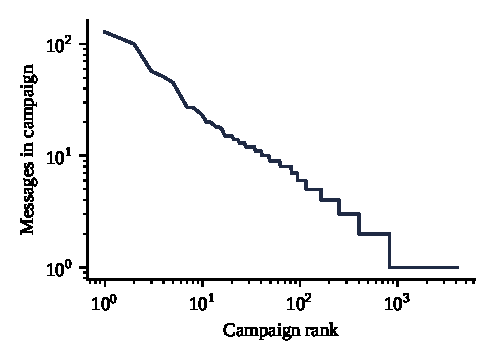
\includegraphics[width=0.82\linewidth]{figures/campaigns.pdf}
\caption{Campaign sizes in the real data (log--log). A few templates account for many messages, which is why random splits leak.}
\label{fig:campaigns}
\end{figure}

\section{Detection Method}
\label{sec:method}

\subsection{Preprocessing}
The cleaner first replaces e-mail addresses, then URLs, including bare links such as \texttt{bit.ly/x} that carry no scheme, then phone numbers, with placeholder tokens. It lowercases the text, removes punctuation while keeping Devanagari vowel signs, and replaces remaining numbers with a number token. The tokenizer keeps Latin and Devanagari words, removes a fixed English stop-word list and applies a light suffix stemmer. Devanagari words are kept intact, so Hindi messages contribute features just as English ones do.

\subsection{Representation and classifier}
A message is represented by the concatenation of two TF-IDF~\cite{salton1988term} vectors with sublinear term frequency: word unigrams and bigrams (at most 30,000 features, minimum document frequency 2, maximum 95\%) and character 2--5-grams within word boundaries (at most 60,000 features, minimum document frequency 2). Character n-grams make the model less sensitive to obfuscation such as \textit{K.Y.C}, \textit{bl0cked} or \textit{S I M}, and to the varied spelling of romanised Hindi. After pruning, the vocabulary has 35,148 features. The classifier is $\ell_2$-regularised logistic regression with $C=16$ and balanced class weights, giving
\begin{equation}
p(x)=\sigma\!\left(\mathbf{w}^{\top}\phi(x)+b\right),
\end{equation}
where $\phi(x)$ is the TF-IDF vector. Logistic regression was chosen on the development split (Section~\ref{sec:setup}); its coefficients also give the per-word contributions shown to users.

\subsection{Intent evidence and fusion}
The deployed system adds an interpretable layer. Thirty-one regular expressions detect 26 scam intents (for example, a request for an OTP, a payment to receive money, a KYC deadline, a remote-access app, a legal threat) and ten protective signals (a warning not to share an OTP, an official reporting channel such as 1909 or 1930, a masked-account transaction alert, a pointer to an official app). Intent weights $w_i$ and protective weights $v_j$ were set by hand. Let $E^{+}=\sum_i w_i$ over matched intents, halved when only weak context cues (deadline, impersonation, generic account threat, a link) match, and $E^{-}=\sum_j v_j$ over matched protective signals, halved when $E^{+}\ge 0.5$. The final score is
\begin{equation}
s(x)=\sigma\!\left(\operatorname{clip}(\operatorname{logit}p(x),\,\pm4)+5\,(E^{+}-E^{-})\right),
\end{equation}
capped at 0.15 when the message has the shape of a genuine transaction alert or service notice and contains no blocking cue such as an install request, a payment demand or a call-to-action on a credited amount. The rules also detect a ``decoy'' pattern, in which a message says ``never share your OTP'' and then asks for it. Matched phrases are shown to the user, grouped into the stages hook, pressure, request and cash-out.

As an alternative we also fit the fusion weights: a logistic regression over the classifier logit, binary intent and protective indicators and the two guard flags, trained on out-of-fold classifier probabilities from campaign-grouped five-fold cross-validation.

\subsection{System integration}
Fig.~\ref{fig:arch} shows the deployed system. A Next.js 14 front end sends the message to a FastAPI back end, which runs preprocessing, the classifier and the intent layer in-process, stores results with SQLAlchemy, and returns the score, the matched phrases and a retrieval-based explanation. Training happens offline. The vectorizer and model are versioned in a model registry and loaded once at start-up, and inference never refits them. Algorithm~\ref{alg:infer} summarises inference.

\begin{figure}[t]
\centering
\resizebox{\linewidth}{!}{%
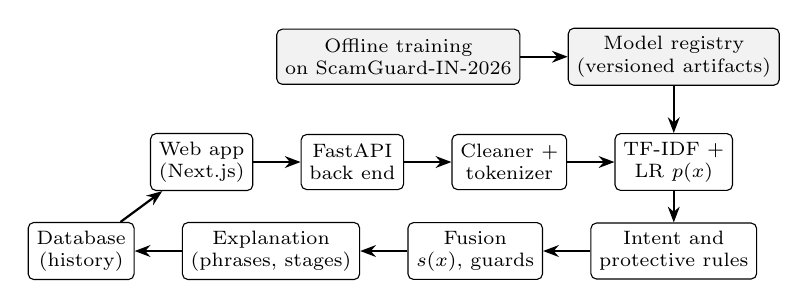
\begin{tikzpicture}[
  node distance=4mm and 6mm,
  box/.style={draw, rounded corners=2pt, align=center, font=\scriptsize, minimum height=7mm, inner sep=3pt, fill=white},
  off/.style={box, fill=gray!10},
  arr/.style={-{Stealth[length=2mm]}, thick}]
\node[box] (ui) {Web app\\(Next.js)};
\node[box, right=of ui] (api) {FastAPI\\back end};
\node[box, right=of api] (pre) {Cleaner +\\tokenizer};
\node[box, right=of pre] (clf) {TF-IDF +\\LR $p(x)$};
\node[box, below=of clf] (rules) {Intent and\\protective rules};
\node[box, left=of rules] (fuse) {Fusion\\$s(x)$, guards};
\node[box, left=of fuse] (expl) {Explanation\\(phrases, stages)};
\node[box, left=of expl] (db) {Database\\(history)};
\node[off, above=6mm of clf] (reg) {Model registry\\(versioned artifacts)};
\node[off, left=of reg] (train) {Offline training\\on ScamGuard-IN-2026};
\draw[arr] (ui) -- (api); \draw[arr] (api) -- (pre); \draw[arr] (pre) -- (clf);
\draw[arr] (clf) -- (rules); \draw[arr] (rules) -- (fuse); \draw[arr] (fuse) -- (expl);
\draw[arr] (expl) -- (db); \draw[arr] (db) -- (ui);
\draw[arr] (train) -- (reg); \draw[arr] (reg) -- (clf);
\end{tikzpicture}}
\caption{System architecture. Shaded boxes run offline; the rest run per request.}
\label{fig:arch}
\end{figure}

\begin{algorithm}[t]
\caption{Scoring one message}
\label{alg:infer}
\footnotesize
\begin{algorithmic}[1]
\Require message $x$; frozen vectorizer $\phi$, weights $\mathbf{w},b$; rules
\State $t \gets \textsc{Tokenize}(\textsc{Clean}(x))$
\State $p \gets \sigma(\mathbf{w}^{\top}\phi(t)+b)$
\State $(I, P) \gets$ matched intents and protective signals in $x$
\If{a sentence asks for an OTP after a ``never share'' warning}
  \State add the decoy intent to $I$; remove the warning from $P$
\EndIf
\State $s \gets \sigma(\operatorname{clip}(\operatorname{logit}p,\pm4)+5(E^{+}(I)-E^{-}(P)))$
\If{$x$ is a genuine alert or notice with no blocking cue} \State $s\gets\min(s,0.15)$ \EndIf
\State \Return $\mathbb{1}[s\ge0.5]$, $s$, matched phrases of $I$ and $P$
\end{algorithmic}
\end{algorithm}

\section{Experimental Setup}
\label{sec:setup}

\textbf{Protocol.} Unless stated otherwise, models are trained on the training and development splits together (9,513 rows, including synthetic data) after model selection on the development split, and evaluated on the real test split: 1,874 messages (665 genuine, 1,209 scam) from campaigns never seen in training. We also report the 259-message development challenge set and the 12-message 2025--26 advisory set; the latter is too small for firm conclusions.

\textbf{Baselines.} We compare Complement Naive Bayes ($\alpha=0.3$), logistic regression ($C=16$), a linear SVM ($C=0.5$, Platt-calibrated by five-fold cross-validation) and a random forest (300 trees), each with word, character and combined features, all from scikit-learn~\cite{pedregosa2011scikit}.

\textbf{Metrics.} With scam as the positive class, a true positive is a scam that is flagged, a false positive is a genuine message that is flagged (a false alarm), and a false negative is a scam that passes. We report accuracy, precision $TP/(TP+FP)$, recall $TP/(TP+FN)$, $F_1=2PR/(P+R)$, the false-alarm rate $FP/(FP+TN)$ and ROC-AUC. Because the cost of a false alarm is high for a tool that asks users to trust their real bank messages, we discuss the false-alarm rate alongside F1. Confidence intervals are 2.5th and 97.5th percentiles of 1,000 bootstrap resamples of the test set. Paired comparisons use the exact McNemar test.

\textbf{Environment.} Python 3.13, scikit-learn 1.7.2, NumPy 2.2.6 and pandas 2.3.3 on a two-core Intel Xeon at 2.8~GHz. Random seed 2026 for experiments and 42 for estimators. All tables come from one script that writes the results to a JSON file.

\section{Results}
\label{sec:results}

\subsection{RQ1: report labels versus audited labels}
Training the same model with every reported message labelled as scam yields a recall of 99.4\% but a false-alarm rate of 34.0\% (95\% CI 30.5--37.8) on the real test set. With audited labels the false-alarm rate is 2.6\% (1.5--3.9) at a recall of 97.6\% (Fig.~\ref{fig:audit}). Of the paired test predictions, the audited model is right where the report-label model is wrong 210 times, and the converse holds 23 times ($p<10^{-30}$). Report labels teach the model that any bank-like message is a scam, which is precisely the failure users notice.

\begin{figure}[t]
\centering
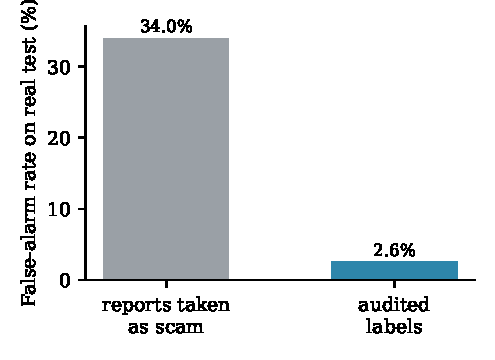
\includegraphics[width=0.78\linewidth]{figures/label_audit.pdf}
\caption{False-alarm rate on the real test set when the same model is trained with report labels or with audited labels.}
\label{fig:audit}
\end{figure}

\subsection{RQ2: random versus campaign-aware split}
On the real data alone, a random 75/25 split places 793 test rows in a campaign that also occurs in training. Under that split, logistic regression scores an F1 of 98.3\% (97.7--98.8) with a 0.8\% false-alarm rate. Under the campaign-aware split it scores 97.7\% (97.1--98.3) with 1.4\%. The difference in F1 is modest, but the false-alarm rate nearly doubles once memorised templates are removed. The random split therefore understates the error that matters most for this application.

\subsection{RQ3: models and features}
Table~\ref{tab:models} compares the baselines. Combined word and character features give the best or near-best F1 for every linear model. Logistic regression with combined features has the lowest false-alarm rate among the strong models (2.6\%). The linear SVM has a slightly higher F1 (98.2\%) but a false-alarm rate of 3.9\%, and the random forest generalises poorly to the challenge messages. We selected logistic regression on the development split, where it and the SVM were within one point of each other.

\begin{table}[t]
\centering
\caption{Real test set (n = 1,874), classifier only. F1 and false-alarm rate (FAR) in \%; ``Ch.'' is F1 on the 259 challenge messages.}
\label{tab:models}
\footnotesize
\begin{tabular}{@{}llrrr@{}}
\toprule
Model & Features & F1 & FAR & Ch. \\
\midrule
Naive Bayes & word & 96.2 & 6.2 & 88.0 \\
 & word+char & 95.5 & 6.5 & 86.6 \\
Logistic regression & word & 98.0 & 2.7 & 89.9 \\
 & char & 96.9 & 4.8 & 86.8 \\
 & word+char & \textbf{98.1} & \textbf{2.6} & 90.2 \\
Linear SVM & word & 97.7 & 5.6 & 91.6 \\
 & word+char & \textbf{98.2} & 3.9 & \textbf{92.0} \\
Random forest & word & 97.5 & 2.7 & 73.7 \\
 & word+char & 97.6 & 3.3 & 73.9 \\
\bottomrule
\end{tabular}
\end{table}

\subsection{RQ4: synthetic data}
Table~\ref{tab:train} varies the training data. A model trained only on synthetic messages reaches 87.4\% F1 on real messages but flags 31.1\% of genuine ones, which shows that templates alone do not capture real Indian SMS. A model trained only on real data performs well on the real test set (97.7\% F1, 1.4\% false alarms) but recognises only 35.6\% of the scams in the challenge set, which covers 2025--26 scam types that the 2017--2024 reports rarely contain. Combining both keeps real-data F1 at 98.1\% and raises challenge F1 from 51.2\% to 90.2\%, at the cost of a higher false-alarm rate on real data (2.6\% against 1.4\%). The synthetic data buys coverage of new scam types with a small loss in precision on older real messages.

\begin{table}[t]
\centering
\caption{Effect of the training data (logistic regression, word+char). Values in \%.}
\label{tab:train}
\footnotesize
\begin{tabular}{@{}lrrrr@{}}
\toprule
Training data & Real F1 & Real FAR & Ch. recall & Ch. F1 \\
\midrule
Synthetic only & 87.4 & 31.1 & 86.4 & 90.3 \\
Real only & 97.7 & 1.4 & 35.6 & 51.2 \\
Real + synthetic & \textbf{98.1} & 2.6 & 82.2 & 90.2 \\
\bottomrule
\end{tabular}
\end{table}

\subsection{RQ5: rules and fusion}
Table~\ref{tab:fusion} compares the classifier, the hand-weighted rules of Section~\ref{sec:method} and learned fusion weights. On the independent real test set, the hand-weighted rules lower F1 from 98.1\% to 97.7\% and raise the false-alarm rate from 2.6\% to 3.2\%. Learned fusion is the best of the three (98.3\%, 2.3\%), and it beats the hand-weighted rules significantly (15 against 2 discordant pairs, $p=0.002$), although not the classifier alone ($p=0.34$). On the challenge set, written by the same people who wrote the rules, the ordering reverses: the hand-weighted rules lift F1 from 90.2\% to 95.6\%. Evaluating rules on messages written by their authors therefore overstates their value. Some learned weights are also instructive. The KYC-demand intent receives a negative weight ($-1.35$), because real Indian banks send many KYC reminders that the rules treat as risky. Prize, pay-to-receive and account-threat intents receive the largest positive weights.

We keep the hand-weighted rules in the deployed system for two reasons. They are the source of the phrase-level explanations shown to users, and they are the only defence against 2025--26 scam types that are absent from the real training data, which the challenge and advisory sets suggest but cannot yet establish.

\begin{table}[t]
\centering
\caption{Classifier alone and two fusion schemes. Values in \%.}
\label{tab:fusion}
\footnotesize
\begin{tabular}{@{}lrrrr@{}}
\toprule
 & \multicolumn{2}{c}{Real test (1,874)} & \multicolumn{2}{c}{Challenge (259)} \\
System & F1 & FAR & F1 & FAR \\
\midrule
Classifier only & 98.1 & 2.6 & 90.2 & 0.0 \\
Hand-weighted rules (deployed) & 97.7 & 3.2 & \textbf{95.6} & 0.0 \\
Learned fusion & \textbf{98.3} & \textbf{2.3} & 91.2 & 0.0 \\
\bottomrule
\end{tabular}
\end{table}

\subsection{Deployed system}
Table~\ref{tab:final} reports all metrics of the deployed system on the real test set, next to the classifier alone and the learned fusion of Section~\ref{sec:method}. The deployed system reaches 97.1\% accuracy (95\% CI 96.3--97.8), 98.2\% precision and 97.2\% recall, with a false-alarm rate of 3.2\% (2.0--4.6). On the 12 advisory messages from 2025--26 it detects 10 of the 11 scams and passes the one genuine operator notice, an F1 of 95.2\%; the set is too small for a firm conclusion.

\begin{table}[t]
\centering
\caption{Real test set (n = 1,874): all metrics in \%, ROC-AUC as a fraction.}
\label{tab:final}
\footnotesize
\setlength{\tabcolsep}{4pt}
\begin{tabular}{@{}lrrrrrr@{}}
\toprule
System & Acc. & Prec. & Rec. & F1 & FAR & AUC \\
\midrule
Classifier only & 97.5 & 98.6 & 97.6 & 98.1 & 2.6 & 0.997 \\
Deployed (hand rules) & 97.1 & 98.2 & 97.2 & 97.7 & 3.2 & 0.995 \\
Learned fusion & \textbf{97.8} & \textbf{98.7} & \textbf{97.8} & \textbf{98.3} & \textbf{2.3} & 0.997 \\
\bottomrule
\end{tabular}
\end{table}

\subsection{Operating point, errors and cost}
The deployed score has a ROC-AUC of 0.995 and an average precision of 0.997 on the real test set (Fig.~\ref{fig:rocpr}). At the 0.5 threshold it misses 34 of 1,209 scams and flags 21 of 665 genuine messages (Fig.~\ref{fig:conf}a). Raising the threshold to 0.9 lowers the false-alarm rate to 0.8\% while recall falls to 92.5\% (Fig.~\ref{fig:conf}b). The false alarms are concentrated in reported-but-genuine bank messages (15 of 240 flagged), many of which ask the user to click a link to complete KYC or a card application, and are rare among personal and promotional messages (6 of 420). Recall is 97.7\% on banking scams (895 of 916) and 92.3\% on government-themed scams (24 of 26).

To measure robustness, we obfuscated 837 test scams that contained keywords such as KYC, PAN, OTP or SIM, using dotted, spaced and digit-substituted spellings. Recall fell from 99.4\% to 98.9\% with word features alone and to 99.3\% with combined features. The character n-grams help, but the effect on this test is small.

The model and vectorizer occupy 0.28~MB and 1.29~MB. Training takes 2.7~s. Scoring one message takes 1.7~ms for the classifier and 3.8~ms including the intent layer on the hardware above.

\begin{figure*}[t]
\centering
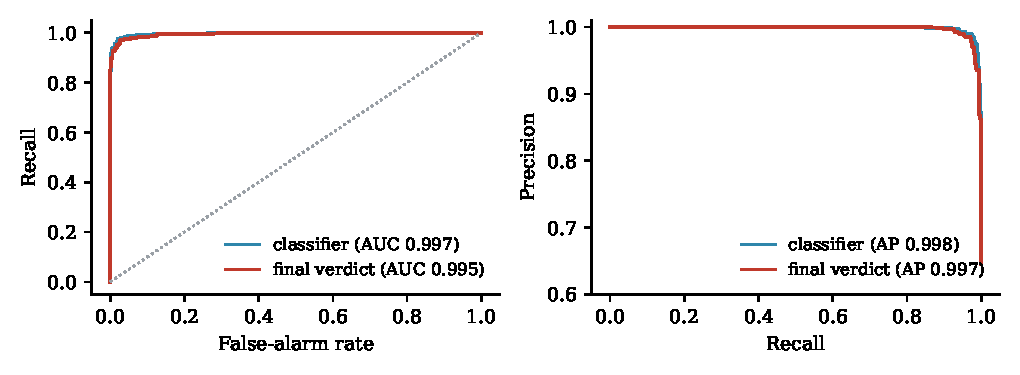
\includegraphics[width=0.78\textwidth]{figures/roc_pr.pdf}
\caption{ROC and precision--recall curves of the classifier and the deployed score on the real test set.}
\label{fig:rocpr}
\end{figure*}

\begin{figure}[t]
\centering
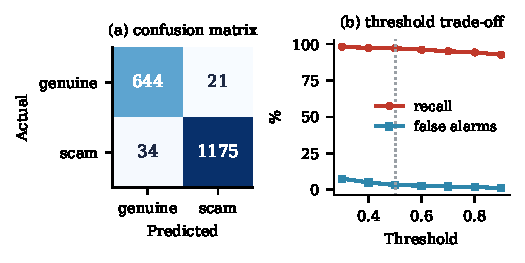
\includegraphics[width=\linewidth]{figures/confusion.pdf}
\caption{Deployed score on the real test set: (a) confusion matrix at threshold 0.5, (b) recall and false-alarm rate as the threshold changes.}
\label{fig:conf}
\end{figure}

\section{Discussion}
\label{sec:discussion}

The clearest result is that the labels matter more than the model. Every linear model we tried reached an F1 between 95\% and 98\% under the same protocol, while the choice between report labels and audited labels moved the false-alarm rate by more than thirty points. The IMC~2025 authors already warned that reports are unverified~\cite{agarwal2025fishing}, and the UK study by the same group found that over a third of reported texts were spam rather than scams~\cite{agarwal2026overview}. Our audit adds a figure for genuine messages among Indian reports and shows its cost when such data is used for training.

The leakage result is smaller than we expected in F1 and larger in false alarms. Most campaigns in the audited data are singletons, so a random split leaks only part of the test set. The leaked part, however, consists of the large template families that the model can memorise, and removing them exposes the harder genuine messages.

The rules result should influence how such systems are evaluated. Rules written while looking at example messages fit those examples. On real messages from unseen campaigns, the classifier had already learned most of what the rules encode, and the hand-set weights added false alarms. Learned weights recovered a small gain. We therefore regard the rule layer as an explanation and coverage device, not as an accuracy improvement, until a large real 2025--26 test set shows otherwise.

\section{Threats to Validity and Limitations}
\label{sec:limits}

\textit{Time coverage.} R1 messages are mostly from 2022--2024. The 2025--26 scam types are represented in training only by synthetic messages and in testing by 12 advisory messages, many of which are illustrative examples from articles rather than received messages. The author-contributed 2026 test set (R4) will address this, and its results are not part of this paper.

\textit{Label reliability.} One annotator made the manual decisions, so we cannot report inter-annotator agreement. Unclear messages were dropped rather than guessed, which may make the test set slightly easier than real traffic.

\textit{Synthetic data.} Templates are cleaner than real text. They raise the false-alarm rate on real data (Table~\ref{tab:train}), and they share authors with the rules and the challenge set.

\textit{Representativeness.} The genuine class comes from two sources and is smaller than the scam class. Personal chat in R2 is mostly work messages. Languages other than English and Hindi are not covered.

\textit{Adversarial robustness.} Our obfuscation test uses simple substitutions. Adaptive attackers, paraphrasing with language models, and scams without any fraud keyword were not tested.

\textit{Single-message scope.} Sender identifiers, conversation history and URL reputation are not used by the classifier, although the application checks links separately.

\section{Ethical and Security Considerations}

The public sources are used under their licences, and IMC~2025 messages were already anonymised by their publishers. Author-contributed messages are masked before storage: OTPs, account and card numbers, phone numbers, UPI identifiers, e-mail addresses and names are replaced, and raw exports are never committed. No institutional ethics review was sought for this work, and no personal data of third parties is released. The detector's score is a risk estimate, not proof of fraud. A false alarm can cause a user to ignore a real bank message, and a missed scam can cause financial loss, so the application shows the evidence behind each verdict, links to the official reporting channels (1930 and cybercrime.gov.in) and tells users to verify through official apps. Releasing the rules may help attackers evade them; we consider the benefit of reproducibility to outweigh this, because the rules encode well-known advisory guidance.

\section{Conclusion}
\label{sec:conclusion}

We studied SMS scam detection for Indian users with a corpus built for that purpose. Auditing user reports showed that one in five retained Indian reports was a genuine message, and that training on report labels raises false alarms from 2.6\% to 34.0\%. Splitting by campaign removes memorised templates and nearly doubles the measured false-alarm rate compared with a random split. A small logistic-regression model over word and character TF-IDF reaches 98.1\% F1 on held-out real messages and runs in milliseconds. Hand-weighted intent rules help explanation and coverage but not accuracy on independent data, a fact that tests on the developers' own messages hide. The deployed system reaches 97.1\% accuracy on real messages from unseen campaigns with a 3.2\% false-alarm rate. The main open issue is a large, real 2025--26 test set, which we are collecting, together with multilingual coverage and adaptive-attack evaluation.

\section*{Data and Code Availability}
The corpus, audit files, build script and experiment code are in the project repository (\url{https://github.com/priyamthakur275/ScamGuard-AI}, directory \texttt{backend/ml\_training}). Raw source files can be downloaded with the included script.

\begin{thebibliography}{99}

\bibitem{agarwal2025fishing}
S. Agarwal, A. Papasavva, G. Suarez-Tangil, and M. Vasek, ``Fishing for smishing: Understanding SMS phishing infrastructure and strategies by mining public user reports,'' in \textit{Proc. ACM Internet Measurement Conf. (IMC '25)}, Madison, WI, USA, 2025, doi: 10.1145/3730567.3764431.

\bibitem{agarwal2026overview}
S. Agarwal, G. Suarez-Tangil, and M. Vasek, ``An overview of 7726 user reports: Uncovering SMS scams and scammer strategies,'' in \textit{Proc. Network and Distributed System Security Symp. (NDSS)}, San Diego, CA, USA, 2026. [Online]. Available: https://arxiv.org/abs/2508.05276

\bibitem{pritom2026sms}
M. M. A. Pritom, S. M. Sanjari, M. Mia, A. M. Shibli, S. M. M. Hossain, M. Ismail, and S. Xu, ``Short message service (SMS) phishing attacks and defenses: A systematic review,'' arXiv:2604.11429, Apr. 2026.

\bibitem{almeida2011contributions}
T. A. Almeida, J. M. Gómez Hidalgo, and A. Yamakami, ``Contributions to the study of SMS spam filtering: New collection and results,'' in \textit{Proc. 11th ACM Symp. Document Engineering (DocEng)}, Mountain View, CA, USA, 2011, pp. 259--262.

\bibitem{almeida2013towards}
T. A. Almeida, J. M. Gómez Hidalgo, and T. P. Silva, ``Towards SMS spam filtering: Results under a new dataset,'' \textit{Int. J. Information Security Science}, vol. 2, no. 1, pp. 1--18, 2013.

\bibitem{roy2020deep}
P. K. Roy, J. P. Singh, and S. Banerjee, ``Deep learning to filter SMS spam,'' \textit{Future Generation Computer Systems}, vol. 102, pp. 524--533, Jan. 2020.

\bibitem{mishra2020smishing}
S. Mishra and D. Soni, ``Smishing Detector: A security model to detect smishing through SMS content analysis and URL behavior analysis,'' \textit{Future Generation Computer Systems}, 2020.

\bibitem{sonowal2018smidca}
G. Sonowal and K. S. Kuppusamy, ``SmiDCA: An anti-smishing model with machine learning approach,'' \textit{The Computer Journal}, vol. 61, no. 8, pp. 1143--1157, Aug. 2018, doi: 10.1093/comjnl/bxy039.

\bibitem{goel2024ml}
D. Goel, H. Ahmad, A. K. Jain, and N. K. Goel, ``Machine learning driven smishing detection framework for mobile security,'' arXiv:2412.09641, Dec. 2024.

\bibitem{timko2024smishing}
D. Timko and M. L. Rahman, ``Smishing Dataset I: Phishing SMS dataset from Smishtank.com,'' in \textit{Proc. 14th ACM Conf. Data and Application Security and Privacy (CODASPY '24)}, Porto, Portugal, 2024, doi: 10.1145/3626232.3653282.

\bibitem{ali2025moz}
F. D. M. A. Ali, S. M. Saide, R. Sousa-Silva, and H. Lopes Cardoso, ``MOZ-Smishing: A benchmark dataset for detecting mobile money frauds,'' in \textit{Proc. 6th Workshop on African Natural Language Processing (AfricaNLP)}, Vienna, Austria, 2025, pp. 158--166, doi: 10.18653/v1/2025.africanlp-1.23.

\bibitem{labonne2023spamt5}
M. Labonne and S. Moran, ``Spam-T5: Benchmarking large language models for few-shot email spam detection,'' arXiv:2304.01238, 2023.

\bibitem{ahmadi2025llm}
M. Ahmadi, M. Khajavi, A. Varmaghani, A. Ala, K. Danesh, and D. Javaheri, ``Leveraging large language models for cybersecurity: Enhancing SMS spam detection with robust and context-aware text classification,'' arXiv:2502.11014, Feb. 2025.

\bibitem{northcutt2021confident}
C. Northcutt, L. Jiang, and I. Chuang, ``Confident learning: Estimating uncertainty in dataset labels,'' \textit{J. Artificial Intelligence Research}, vol. 70, pp. 1373--1411, 2021, doi: 10.1613/jair.1.12125.

\bibitem{lee2022dedup}
K. Lee, D. Ippolito, A. Nystrom, C. Zhang, D. Eck, C. Callison-Burch, and N. Carlini, ``Deduplicating training data makes language models better,'' in \textit{Proc. 60th Annu. Meeting Assoc. Computational Linguistics (ACL)}, Dublin, Ireland, 2022, pp. 8424--8445, doi: 10.18653/v1/2022.acl-long.577.

\bibitem{kapoor2023leakage}
S. Kapoor and A. Narayanan, ``Leakage and the reproducibility crisis in machine-learning-based science,'' \textit{Patterns}, 2023, doi: 10.1016/j.patter.2023.100804.

\bibitem{broder1997resemblance}
A. Z. Broder, ``On the resemblance and containment of documents,'' in \textit{Proc. Compression and Complexity of SEQUENCES 1997}, Positano, Italy, 1997, doi: 10.1109/SEQUEN.1997.666900.

\bibitem{salton1988term}
G. Salton and C. Buckley, ``Term-weighting approaches in automatic text retrieval,'' \textit{Information Processing \& Management}, vol. 24, no. 5, pp. 513--523, 1988, doi: 10.1016/0306-4573(88)90021-0.

\bibitem{pedregosa2011scikit}
F. Pedregosa \textit{et al.}, ``Scikit-learn: Machine learning in Python,'' \textit{J. Machine Learning Research}, vol. 12, pp. 2825--2830, 2011.

\end{thebibliography}

\end{document}
